In this section, we describe the design of \scheme{} as a timing-based defense against NUCA side-channel attacks.

\subsection{Network-on-Chip and Router Bypass} \label{sec-noc-background}
Network-on-chip (NoC) has become a scalable communication fabric for large-scale NUCA architectures.
In a NoC, Network Interfaces (NIs) connect each core/cache tile to the network through a set of routers.
A packet travels from the NI of the source tile through the network routers to the NI of the destination tile.
A router consists of several pipeline stages, including routing computation, virtual channel allocation, switch arbitration, and switch traversal, followed by link traversal.
Consequently, packets traverse the network hop-by-hop through a multi-stage router pipeline.

To reduce packet latency, router bypassing has been proposed in various forms~\cite{krishna2013breaking}.
Express Virtual Channels (EVCs) virtually bridge two nodes across multiple bypass routers so that a packet traverses a bypass router in one cycle, without virtual channel or switch arbitration.
Building on EVC, SMART~\cite{krishna2013breaking} enables a single-cycle multi-hop data path from source to destination.
In this work, we leverage the bypass mechanism to selectively regulate packet latency for mitigating NUCA attacks (Section~\ref{sec-bscheme}).
This is the \emph{first} use of a bypass mechanism to resolve a distance-based NUCA cache side-channel attack.

\subsection{Scope of \scheme} \label{sec-scope}
We now explain which memory accesses \scheme{} targets and why.

\scheme{} is applied only to accesses that cause LLC hits.
Accesses that hit in L1D never reach the LLC and are therefore unaffected by LLC bank distances.
Accesses that miss in the LLC incur DRAM latency, which dominates any NoC traversal difference and cannot be exploited for a distance-based or congestion-based NUCA attack.
We refer to any load instruction that causes an LLC hit as a \emph{Security Sensitive} instruction, also called a Secure LD.

\scheme{} does not target store instructions for two reasons.
First, from the perspective of an attacker, a store instruction is harder to time due to write buffers and the inability to use fence instructions freely.
Second, an attacker cannot enforce LLC hits for store instructions: when the attacker brings a cache line to the LLC and the victim later stores to it, the store generates coherence invalidations rather than an LLC hit, making a NUCA attack infeasible.

\subsubsection{Defending Against Congestion-Based Attacks}
Congestion-based attacks rely on observable latency increases caused by deliberate NoC congestion on the communication path of the victim~\cite{meshup,dont-mess-around}.
To defend against these attacks, \scheme{} ensures that all packets are delivered within a fixed latency bound regardless of congestion.
Setting this bound to $T_{worst}$ provides security but hurts performance (Section~\ref{sec:perf-overhead}).
Instead, \scheme{} uses a lower bound $T_{low}$ maintained even in the presence of congestion, as described in Section~\ref{sec-bscheme}.

\subsubsection{Defending Against Distance-Based Attacks}
Distance-based attacks~\cite{mahmud2022distancebased} exploit latency differences between LLC accesses to near and far banks.
Unlike congestion-based attacks, they cannot be resolved by cache partitioning or isolation alone.
\scheme{} eliminates the timing signal by ensuring that all Security Sensitive LLC-hit accesses complete in constant time, regardless of the distance to the target LLC bank or CHA.

\subsection{Overview of \scheme} \label{sec-overview}

\begin{figure}[t]
    \centering
    \includegraphics[width=\columnwidth]{figs/Camouflage-Overview.pdf}
    \caption{Overview of \scheme{}.
    \scheme{} hardware ensures fixed latency for LLC memory accesses using delay and/or bypass techniques.}
    \label{fig:overview}
\end{figure}

Figure~\ref{fig:overview} shows an overview of \scheme{}.
When a core executes a Security Sensitive instruction, it sends a request to the CHA through the NI.
The CHA determines the destination tile and sends a forwarding request.
\scheme{} hardware at the destination NI checks the expected round-trip latency against the target latency.

\scheme{} chooses the target latency based on either the worst-case round-trip latency to the furthest LLC bank (\jscheme{}) or the minimum achievable round-trip latency to the furthest LLC bank using bypass (\bscheme{}).

With \jscheme{}, the destination NI uses normal routing to send back the response, and the source NI adds the necessary delay upon receiving it.
With \bscheme{}, if the expected round-trip latency exceeds $T_{low}$, the destination NI sends the response through a bypass channel to expedite delivery.
Upon receiving the response, the source NI adds any remaining delay needed to meet $T_{low}$.
In both schemes, \scheme{} hardware ensures constant LLC-hit latency for Security Sensitive instructions, preventing any NUCA timing attack.

\subsection{\jscheme} \label{sec-jscheme}
\jscheme{} is the simplest approach to ensuring constant LLC access latency.
It sets the target latency to the worst-case round-trip latency $T_{worst}$ from the source NI to any destination NI, and delays every response until that time elapses.

For a 2D mesh topology, the worst-case scenario occurs when the source NI is at one corner and the destination NI is at the opposite corner.
Since the worst-case latency varies with network traffic, $T_{worst}$ is determined under a heavily congested but not yet saturated network.

Using Booksim 2.0~\cite{booksim}, we simulate an $8\times8$ mesh and measure round-trip latency at varying injection rates (Figure~\ref{fig:jitter-threshold}).
We set $T_{worst}=100$ cycles, corresponding to the round-trip latency just before network saturation (injection rate 0.357), at which the one-way network latency is under 50 cycles on average.
We do not select a point at or above saturation because at saturation the round-trip latency becomes non-deterministic and prohibitively large, making a distance-based NUCA attack impossible regardless.

\begin{figure}[t]
    \centering
    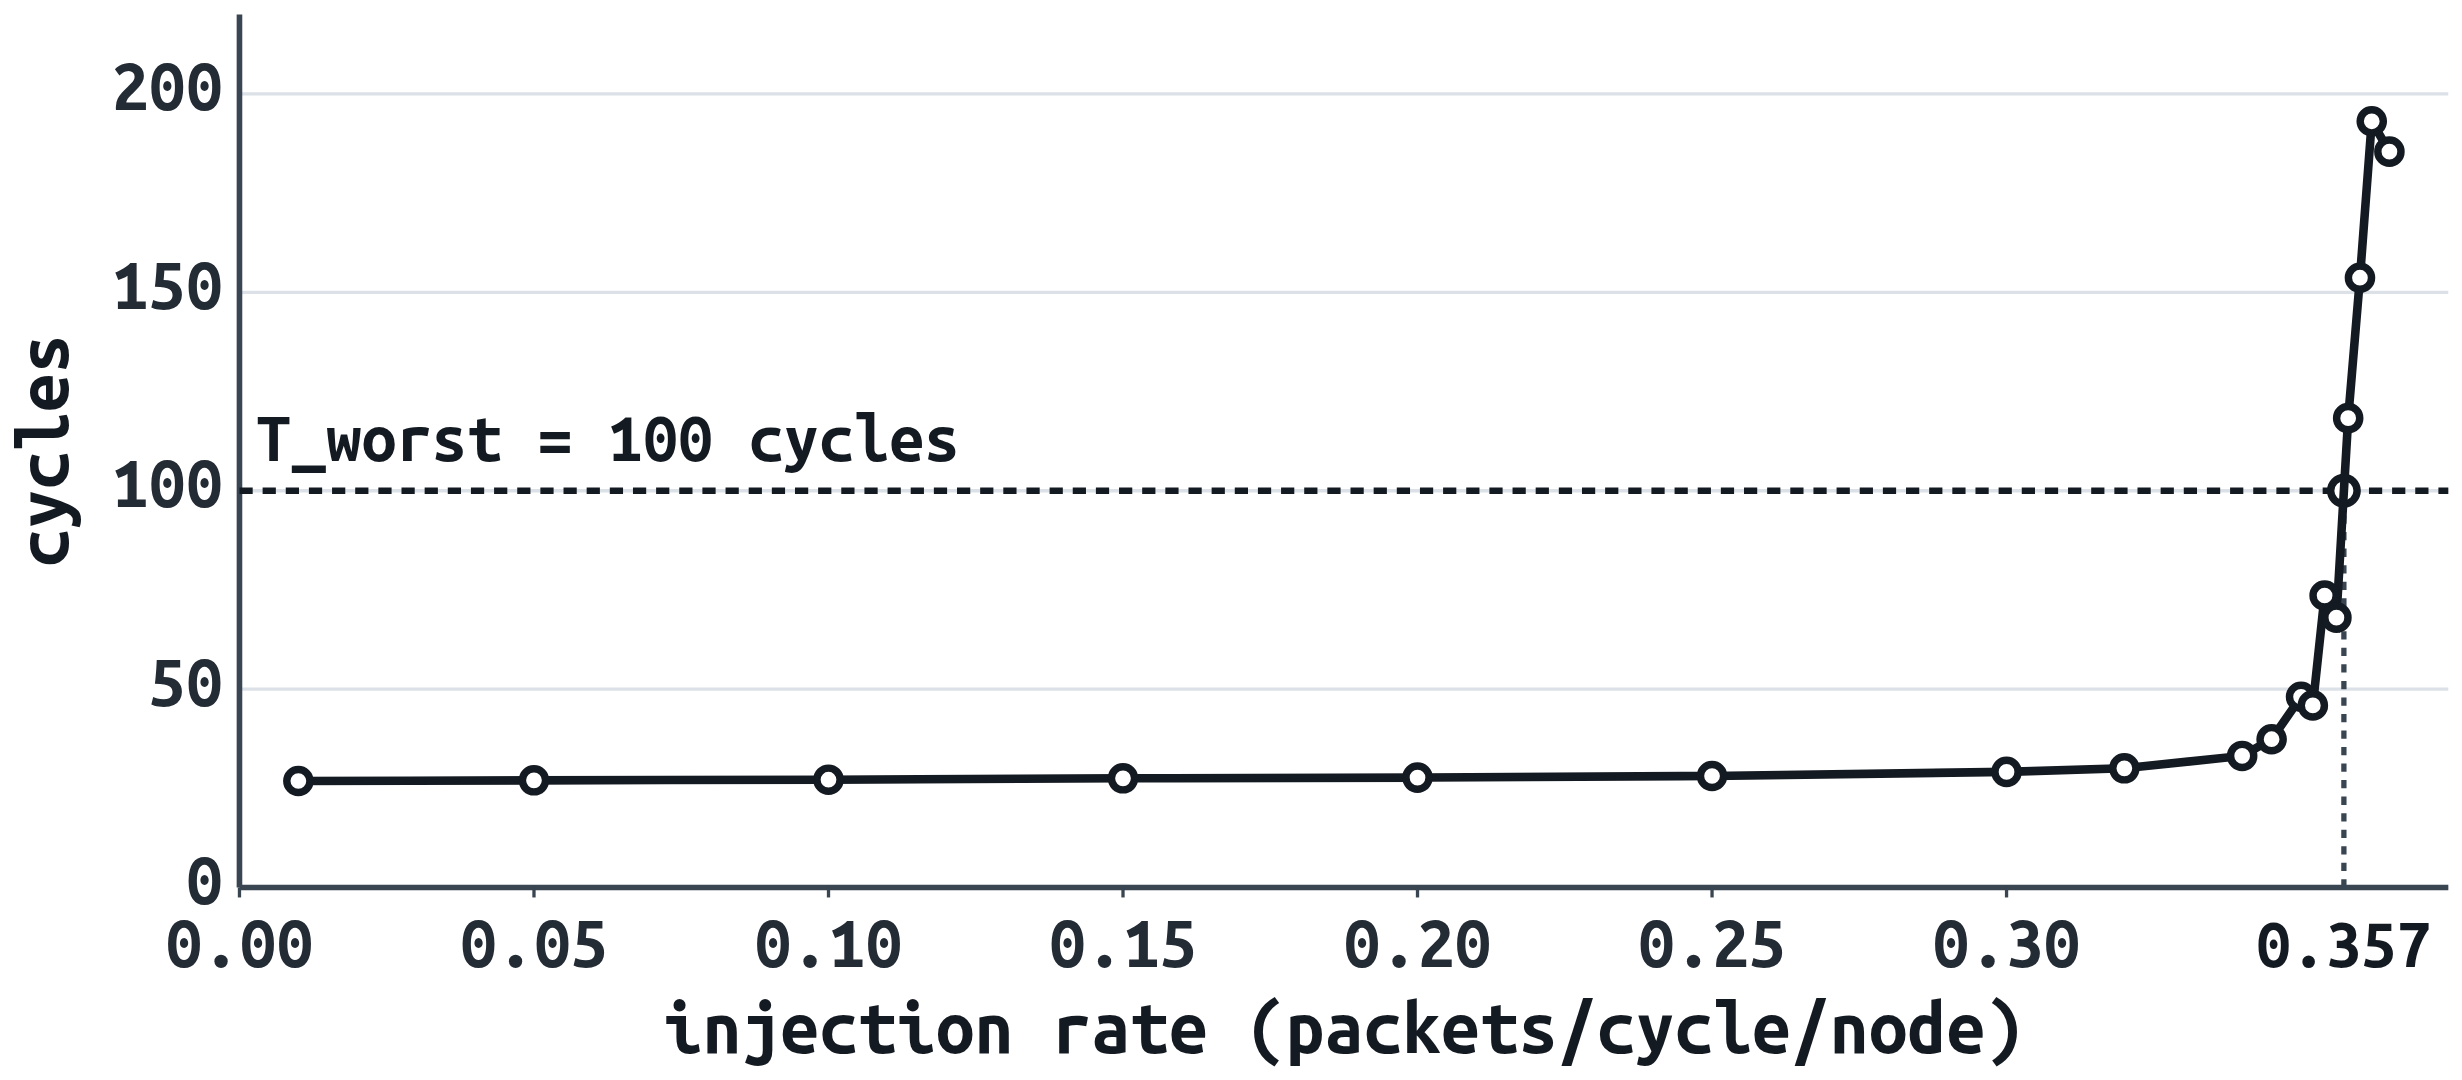
\includegraphics[width=0.95\columnwidth]{figs_new/boundnoc_worst_case_booksim.png}
    %{figs/worst-case-simulation-8x8.pdf}
    \caption{Average network latency of the worst-case (transpose) traffic pattern in an $8\times8$ mesh topology simulated using Booksim~\cite{booksim}.
    The network saturates at injection rate~0.357; we set $T_{worst}=100$ cycles to cover the worst-case round-trip latency just before saturation.}
    \label{fig:jitter-threshold}
\end{figure}

For every Security Sensitive request, the source NI sends the packet through the network and records the actual round-trip latency $T_{orig}$ upon receiving the response.
The source NI then buffers the response in a Delay Queue (DQ) for $T_{worst}-T_{orig}$ cycles before forwarding it to the core.
Thus, \jscheme{} makes every LLC-hit round-trip latency equal to $T_{worst}$, preventing any NUCA timing attack.

\begin{figure}[t]
    \centering
    \includegraphics[width=0.9\linewidth]{figs/NI-updates-v2.pdf}
    \caption{Network Interface extended with a Delay Queue (DQ) and arbitrator (ARB) for \jscheme{}.}
    \label{fig:ni_update}
\end{figure}

\jscheme{} requires minimal hardware changes, as shown in Figure~\ref{fig:ni_update}.
The existing stall queues of the NIs can serve as Delay Queues (DQs) with the addition of multiplexers and an arbitrator (ARB).
Delay is applied only to responses corresponding to LLC hits.
When the destination bank determines that a request causes an LLC miss, it marks the response with a \emph{Delay Required} flag set to \emph{False}.
The source NI skips the delay for such responses and forwards them immediately.

Although \jscheme{} is simple and intuitive, it incurs significant performance overhead because every Security Sensitive LLC-hit access suffers the worst-case latency.
As multicores grow larger, $T_{worst}$ may reach hundreds of cycles, further exacerbating this overhead.
We therefore propose \bscheme{} to reduce this cost.

\subsection{\bscheme} \label{sec-bscheme}
\bscheme{} uses a combination of delay and bypass to achieve both security and performance.
Its goal is to reduce the target round-trip latency from $T_{worst}$ to a lower value $T_{low}$, defined as:
\begin{equation}
\label{eq:tlow}
T_{low} = T_{src \to CHA}^{worst} +
          T_{CHA \to dest}^{worst} +
          T_{dest \to src}^{bypass}
\end{equation}
where $T_{src \to CHA}^{worst}$ and $T_{CHA \to dest}^{worst}$ are the worst-case one-way latencies for those legs, and $T_{dest \to src}^{bypass}$ is the minimum achievable latency from the furthest destination back to the source using router bypass.
We assume the worst case for the first two legs since the attacker controls the source and the requested address, which determines the CHA location.
We choose to expedite only the destination-to-source leg because it carries the actual data, and doing so alone is sufficient to eliminate runtime overhead.

Packets from far destination NIs use bypass to meet $T_{low}$, while packets from nearby NIs use delay.
Algorithm~\ref{alg:defense} details the per-packet decisions made at the source and destination NIs.
Based on the expected round-trip latency $EL_P$~\cite{xiang2016model}, \bscheme{} decides whether to use the bypass channel or regular routing.
If $EL_P > T_{low}$ (Line~11), bypass is used for the response packet.
After the response arrives at the source NI, \bscheme{} checks whether it arrived earlier than $T_{low}$ (Line~17) and adds any remaining delay as needed.

\begin{algorithm}[t]
\footnotesize
\KwData{Sensitive Packet P}
    Src $\leftarrow$ Source NI of the sensitive instruction\;
    Dest $\leftarrow$ Destination NI of the sensitive instruction\;
    $T_{low}$ $\leftarrow$ Target round-trip latency (Equation~\ref{eq:tlow})\;
    $EL_P$ $\leftarrow$ Expected round-trip latency of P from Src to Dest\;
    \If{P is a request packet}{
        Use normal routing protocol for P\;
    }\Else{
        \tcp{P is a response packet from Dest}
        \If{Current NI $=$ Dest}{
            \eIf{$EL_P > T_{low}$}{
                Use bypass for P from Dest to Src\;
            }{
                Use normal routing protocol for P\;
            }
        }\ElseIf{Current NI $=$ Src}{
            $AL_P$ $\leftarrow$ Actual round-trip latency from Src to Dest\;
            \If{$AL_P < T_{low}$}{
                Delay P for $T_{low} - AL_P$ cycles\;
            }
        }
    }
\caption{\bscheme{} packet handling at the NI.}
\label{alg:defense}
\end{algorithm}

To implement bypass, \bscheme{} does not require new physical links.
Instead, one flit-sized buffer is reserved at every router along the bypass path to ensure space for bypassed flits.
This can be extended to support multiple simultaneous flits when multiple NUCA timing attacks occur concurrently.

\bscheme{} also handles congestion-based attacks.
When the source router experiences congestion, it may be unable to forward bypass packets in time.
To detect congestion early, \bscheme{} monitors the credit flow from downstream routers, which indicates the number of free buffers available~\cite{dally1993deadlock,kim2005low,gratz2008regional}.
If no credits are received from a downstream router within a threshold time $T_{cong}$, congestion is assumed on that path.
Upon detecting congestion, \bscheme{} switches from static XY routing to adaptive routing~\cite{duato2001general,gratz2008regional,kim2005low} to avoid the congested path, and combines adaptive routing with bypass to ensure packet delivery within $T_{low}$.
